\chapter{\label{ch:5-results}Results}


This section shows and discusses the results of our experiments based on the models and the datasets introduced in Chapter \ref{ch:4-methods}. It also describes the rationale behind deciding which experiments should be run.

\section{HEXEvent dataset} \label{sec:hexevent_results} %TODO> hexvent dataset section whether the other ones are not
To obtain a baseline, we evaluate the reimplemented and proposed model on the HEXEvent dataset as used in \cite{dsc} and introduced in \ref{subsec:hexevent}. The results of these experiments are shown in Figure \ref{fig:hexevent_auc}.

\subsubsection{Analysis of main findings}
Generally all models perform extremely well with AUCs nearing 90\%. They also perform very similarly, making it hard to differentiate them based on their ROC curves. The Attn model seems to perform slightly better than the other models. 

Assessing our reimplementation, we observe a small difference between the AUC value reported in \cite{dsc} (mean 0.899, standard deviation of 0.18) and the ones we observe (mean 0.873, standard deviation of 0.06). This is likely just a result of random statistical noise influenced by different random seeds between runs and differences between TensorFlow / Keras (their implementation) and PyTorch (our implementation). Notably, when reevaluating the publically available original implementation, in a single run we also obtain results (0.872 AUC) closer to the results of our reimplementation. 
%There is a small (~2\%) difference in the AUC values in the AUC values for the DSC model reported in \cite{dsc} (89.9 AUC) and the ones we observe (87.1 AUC original). 
Thus, we conclude that, albeit with minor caveats, the reimplementation was successful and that we are able to replicate the results of \cite{DSC}.


\begin{figure}
	\centering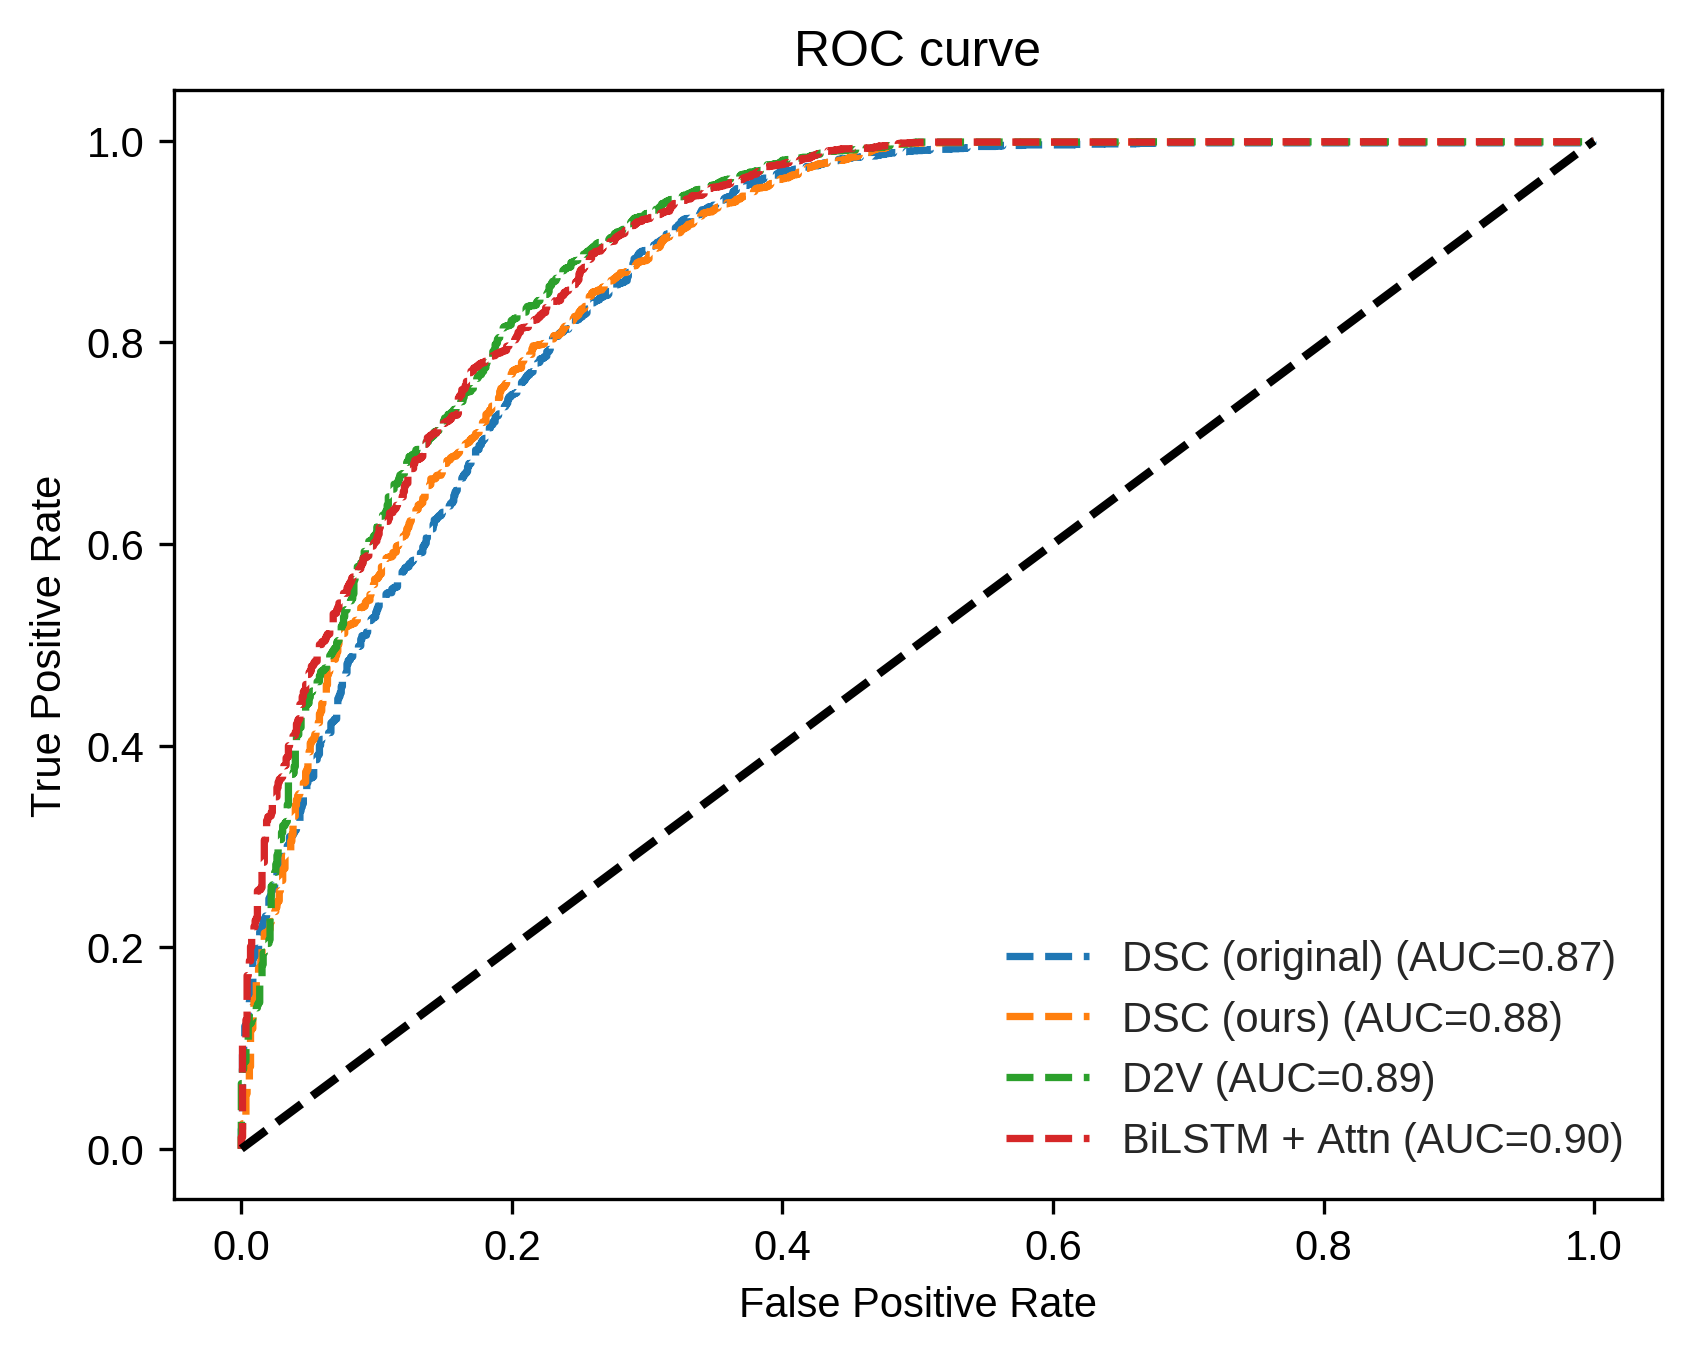
\includegraphics[width=0.7\textwidth]{../visualizations/hexevent_cross_model_roc_auc_comparison.png} 
	\caption[bla.]{Comparison of the ROC curves of the three main models (as well as the original implementation) on the HEXEvent dataset. The values of the original implementation were obtained by rerunning the training on the publicly available implementation. }
	\label{fig:hexevent_auc}
\end{figure}

%main takeaway: all models perform extremely well \& very similarly



%To showcase the advantage of using the attention mechanism, we also included the BiLSTM-based model where only the last output is used for classification. This model performs significantly worse than the other ones.

% Observation: Performance heavily drops when no lengths feature is used

\subsubsection{Length features are necessary}
Reimplementation was done piece-wise, that is, first the sequence features were added as input, then the networks were trained to make sure that this was done correctly and then the length features were added. This lead to an interesting observation: model performance is significantly worse when no length features are given to the models. Quantitative results for this observation are given in table \ref{table:results_hexevent}. This observation is true across models and leads to an average relative performance drop of over 66\%. The information about the secondary structure obtained in the lengths seems to be necessary for the models to obtain good predictive power.

% 0.684, 0.737, 0.663
%0.255, 0.282, 0.268
\begin{table}[h!]
	\centering
	\begin{tabular}{| l | c | c | c| c} 
		\hline
		Model name & Only sequences & Sequences + lengths & Relative performance difference\\
		\hline
		DSC & 0.618 & 0.873 & 0.684\\
		D2V & 0.614 & 0.896 & 0.737\\
		BiLSTM + Attn & \textbf{0.636} & \textbf{0.904} & 0.663\\
		\hline
	\end{tabular}
	\caption{Performance of the main models on the HEXEvent dataset with and without length features given as AUC. Note that the relative performance drop was computed with reference to the baseline AUC value of 0.5.
	}
	\label{table:results_hexevent}
\end{table}

\subsubsection{Further investigations}
To further investigate, we also test three other models: MLP100, MLP20 and MLPLinear which respectively contain 100, 20 and 20 trainable parameters. The models are simple MLPs with one hidden layer which only take the length features as inputs. MLPLinear doesn't use a non-linear activation function after its hidden layer.

Surprisingly, the results in Figure \ref{fig:dsc_funeral} show that it is possible to replicate the results of \cite{dsc} with these very simple models using two to three orders of magnitude fewer parameters. Model performance is improved by adding further parameters and breaks down when no non-linearities are used in the network. This indicates that the models capture a relatively simple, but non-linear relationship between the lengths and the classification of an exon in the dataset. 
There are multiple possible explanations for why this is:
\begin{enumerate}
	\item there are confounders in the dataset learned by the model. As discussed in Section \ref{subsec:hexevent}, EST-based is inherently biased. The biases inherent in EST-based data could be captured by the exon and intron structure and the model is learning to make its prediction based on this bias. This explanation is made more likely, if the findings on the HEXEvent dataset don't replicate on the other datasets we evaluate.
	\item exon splicing is extremely well predictable based on the lengths of neighbouring introns and exons. This is very unlikely given that research into splicing has been going on for over 40 years. This explanation, albeit unlikely already, can be disproven if this observation fails to replicate on other datasets.
	\item there are bugs (e.g. mixing of testing and validation data) in our reimplementation. In the first instance, this is unlikely given that we were able to replicate the original results of \cite{dsc}. To reduce complexity and further reduce the likelihood of a bug leading to these observations, we extracted the complete code for replicating the results of the simple MLP models from \ref{fig:dsc_funeral} into a single file. Additionally, in case of a simple bug the performance of the linear model likely wouldn't break down either. Therefore, we think that this possibility is unlikely. 
\end{enumerate}

Overall, we conclude that the HEXEvent-based dataset is most likely fundamentally flawed and suffers from confounders.
These findings have strong implications. It calls into questions the meaningfulness of \cite{dsc}'s results, showing the competitiveness of their model. These findings likely also warrant a critical investigation of any other conclusions drawn from papers based on the HEXEvent database. At the time of writing, the HEXEvent paper is cited 34 times. While most of these citations are just in passing, there are also multiple papers which use a HEXEvent-derived dataset for the training of Machine Learning models such as SVMs \cite{buschhertel}, Random Forests \cite{flawed1}, Decision Trees \cite{flawed2} or AdaBoost-based algorithms \cite{flawed3}. Due to these data quality issue, we try to construct an alternative dataset.


% many of them, even correlational studies, say that this is a feature, rather than a bug
% how true is this?
% mgith even have to post-pone condemning of HEXEvent dataset until I find a better one 

%Recognition of alternatively spliced cassette exons based on a hybrid model -- confirmed

%A classification of alternatively spliced cassette exons using AdaBoost-based algorithm -- actually says that this is a feature, not a bug

%G2P: Using machine learning to understand and predict genes causing rare neurological disorders --- definitely in some capacity
%Exon size and sequence conservation improves identification of splice-altering nucleotides -- this observation is actually their main contribution
% short exons are more likely to be alternatively spliced


%We showed that the EST-based HEXEvent dataset is likely too flawed to serve as a basis for our methods. Thus, we try to construct an alternative dataset.

%TODO: move figures into directories and update figure links

\begin{figure}
	\centering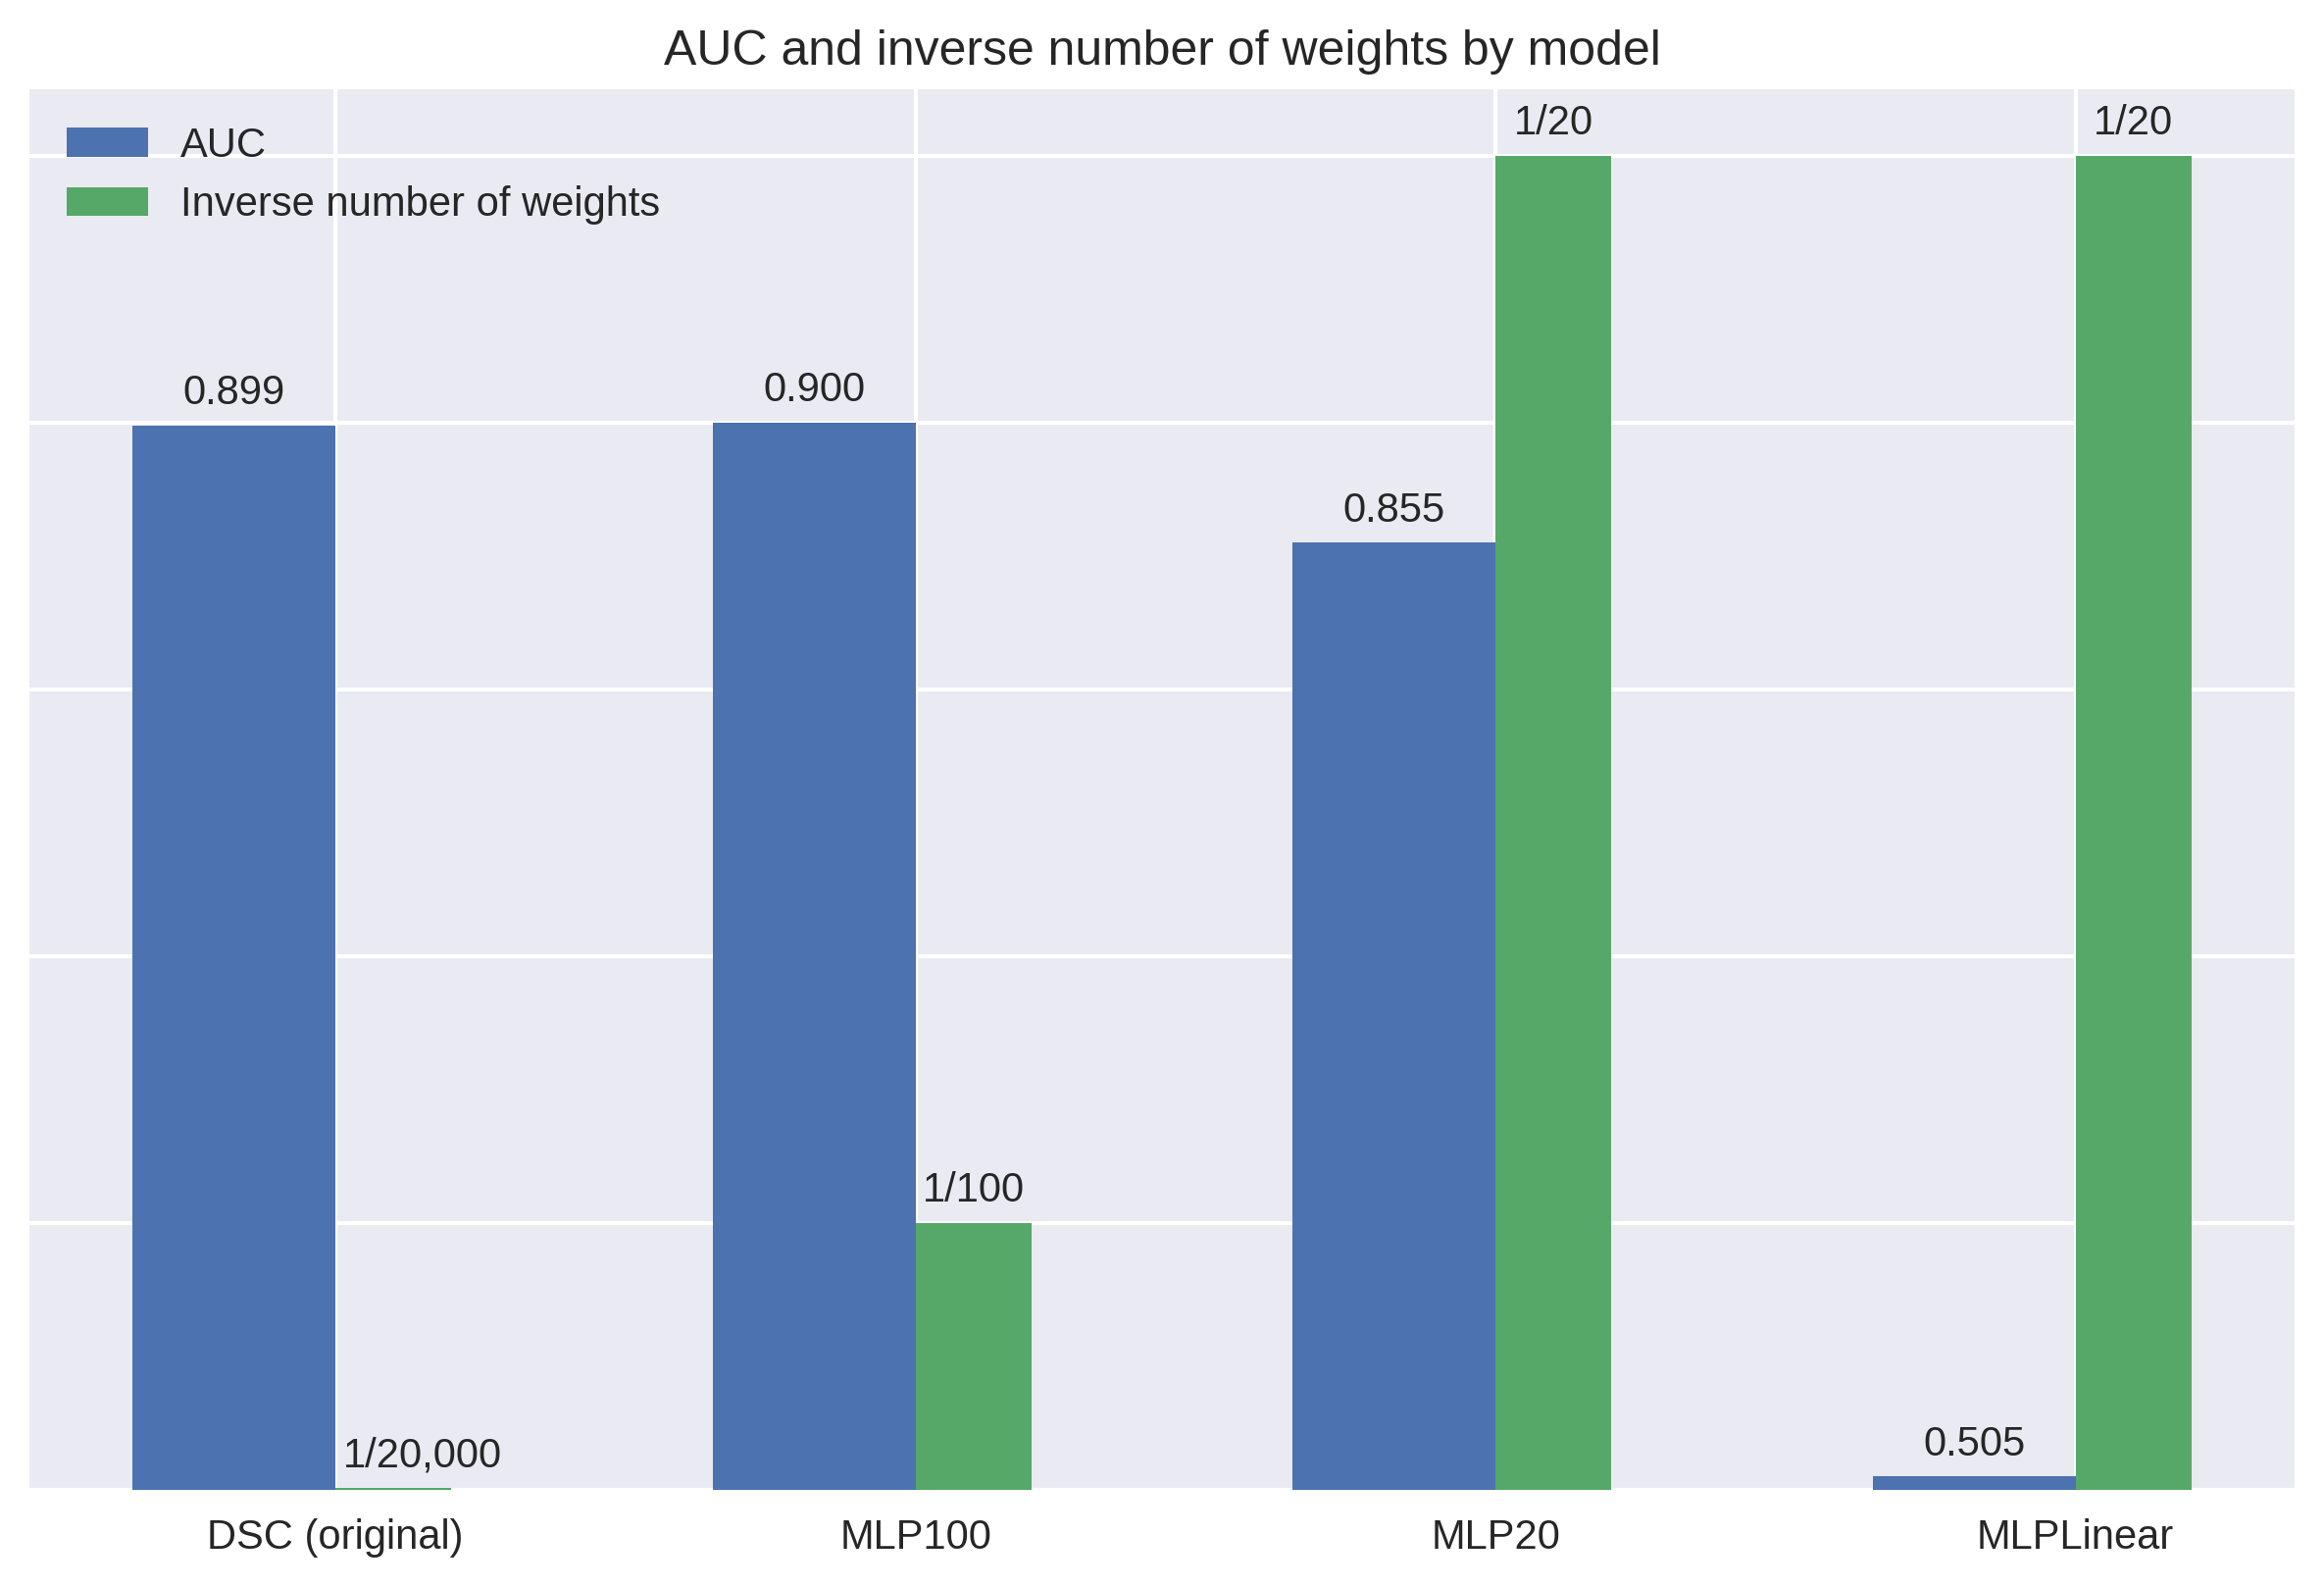
\includegraphics[width=0.7\textwidth]{../visualizations/dsc_funeral_barchart.png} 
	\caption[bla.]{Stress testing the HEXEvent dataset used in \cite{dsc}. The graph shows the performance as well as the inverse of the respective model sizes used.}
	\label{fig:dsc_funeral}
\end{figure}

%TODO: tSNE of MLP embeddings?


\section{GTEx-based datasets} \label{sec:gtex}
\subsection{Cassette exon-based datasets} \label{subsec:gtex_exon}


\begin{figure}
	\centering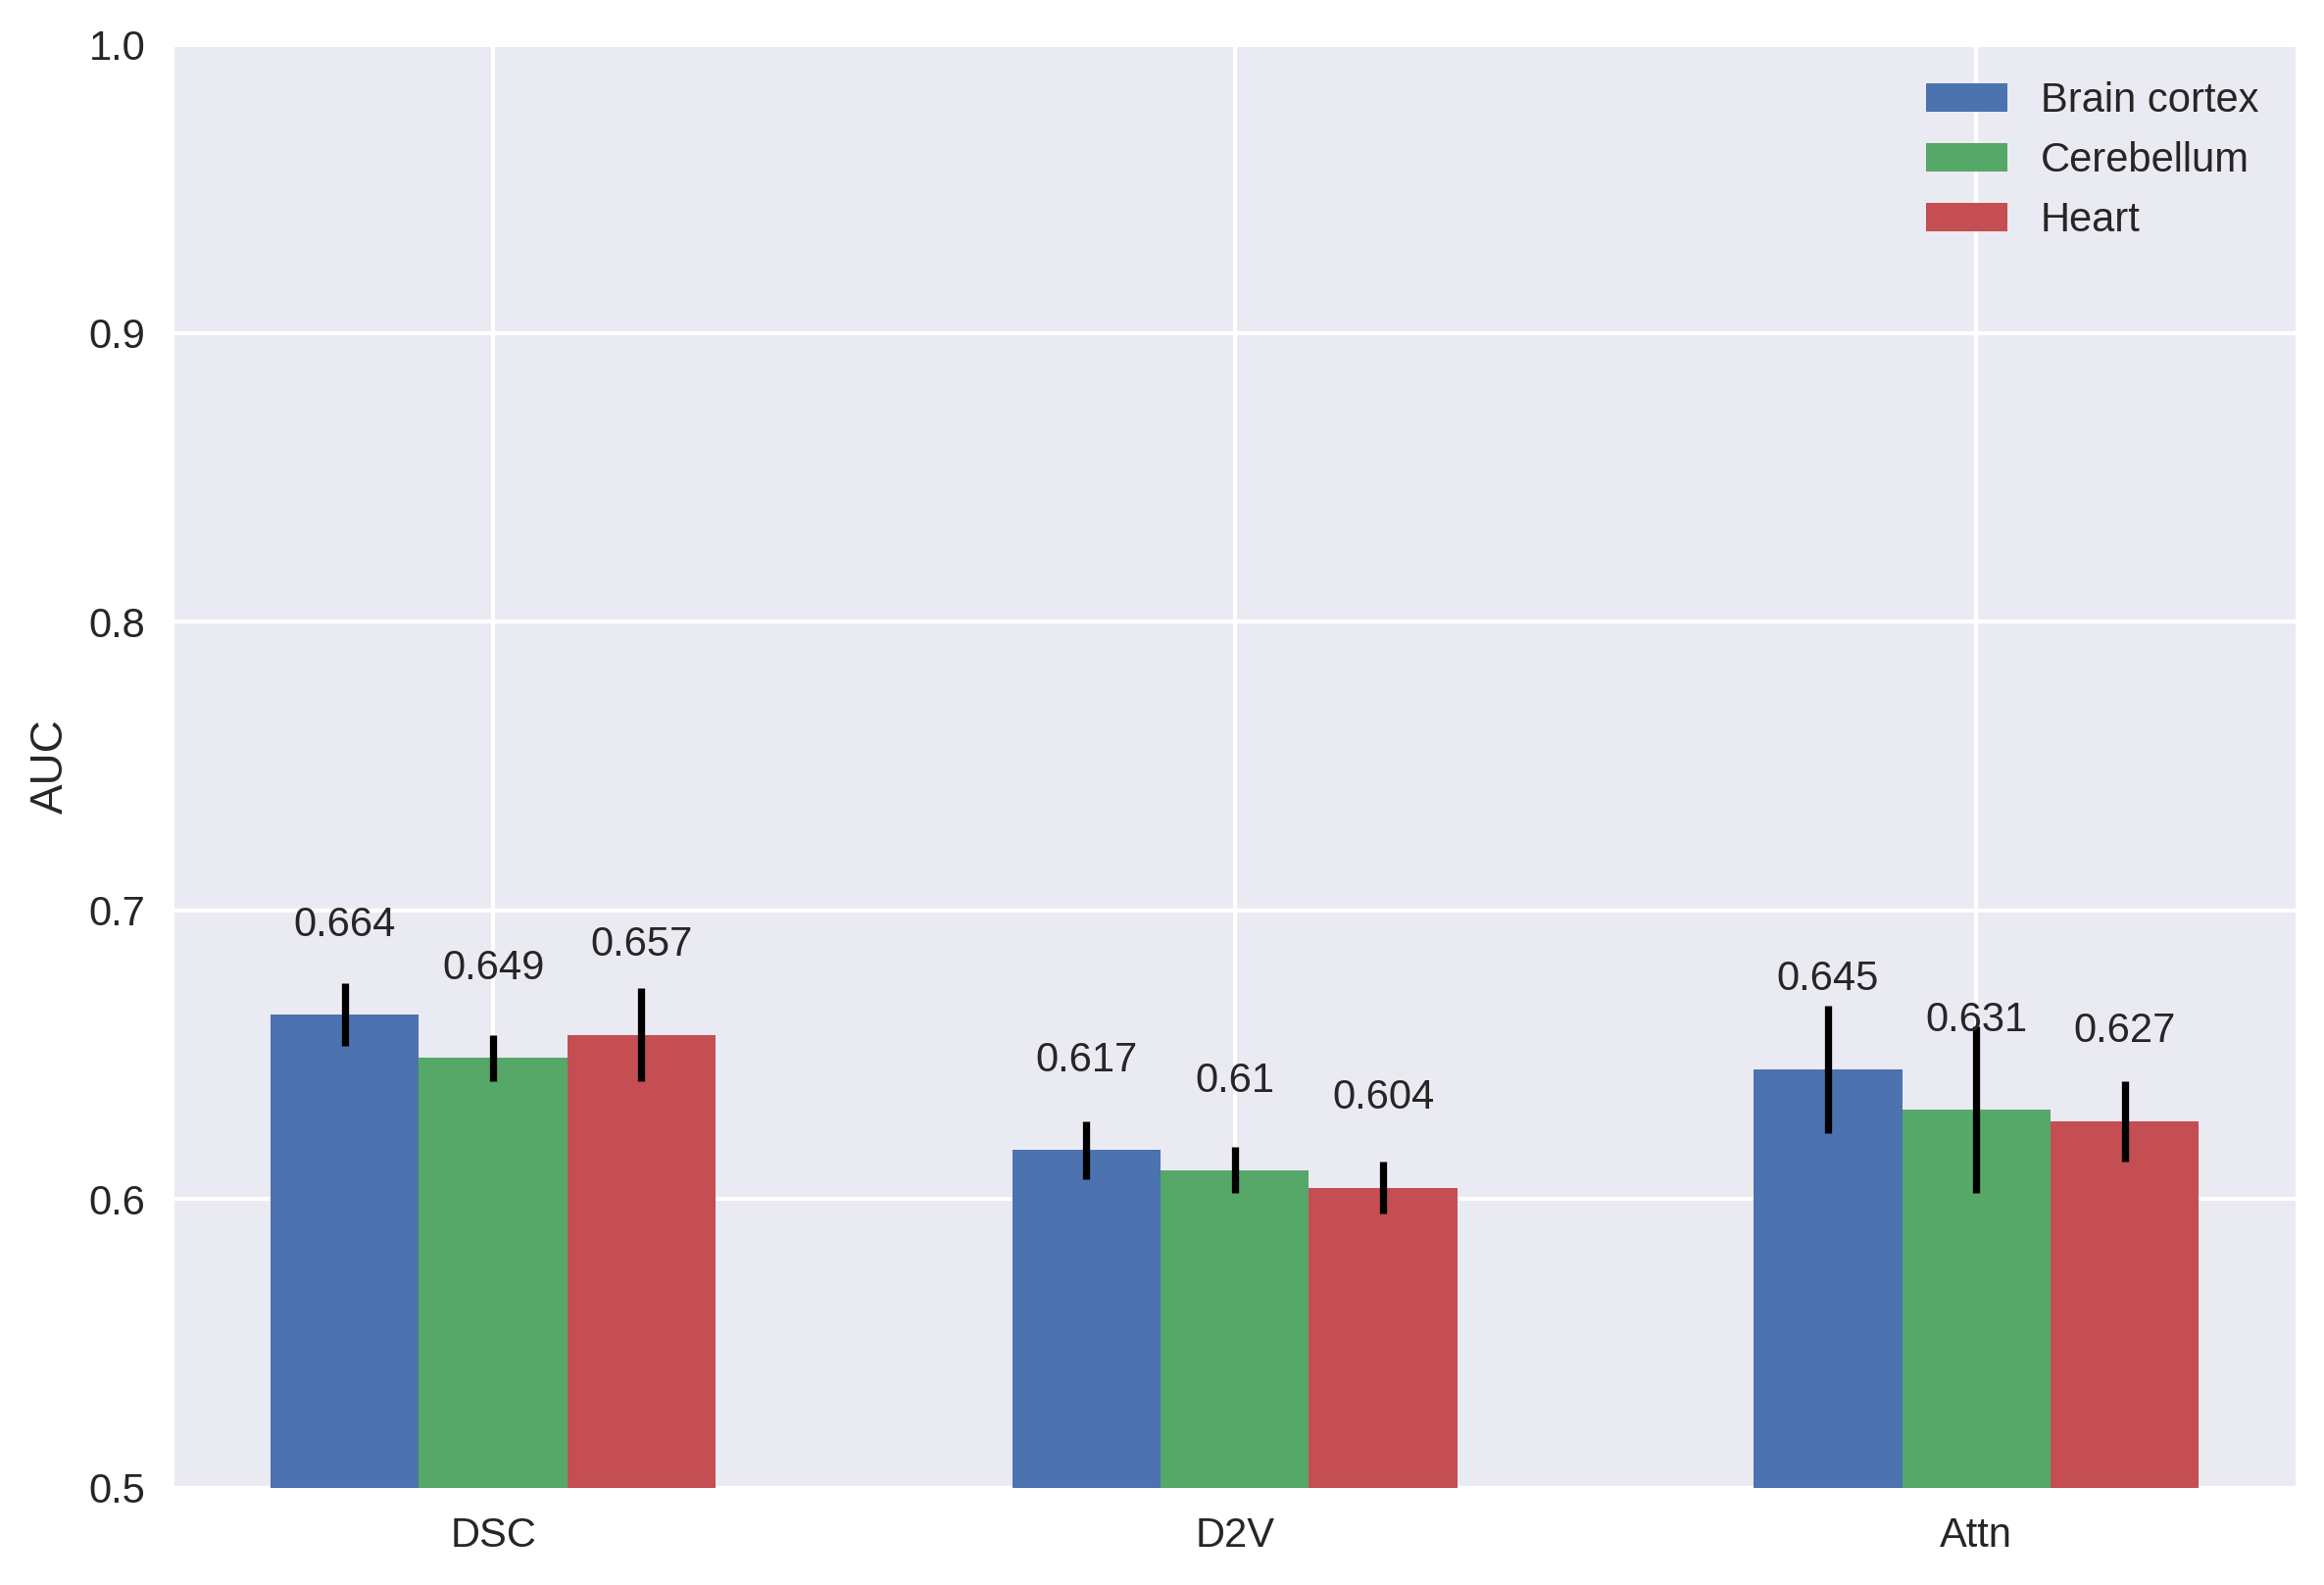
\includegraphics[width=0.7\textwidth]{../visualizations/gtex_exon_barcharts.png} 
	\caption{Performance on the GTEx-based exon datasets for different tissues. The error bars give the standard deviation across all cross-validation runs. }
	\label{fig:gtex_exon_barcharts}
\end{figure}

\begin{figure}
	\centering\includegraphics[width=0.7\textwidth]{../saved/log/GTEx_Exon_Brain_DSC/final/ROC.png} 
	\caption{Bar chart of the performance on the GTEx-based exon datasets for different tissues. The error bars give the standard deviation across all cross-validation runs.  }
	\label{fig:gtex_exon_roc}
\end{figure}

Results are given in Figure (....). Across all models, the performance is poor and the predictive power of the models is low. Surprisingly, performance is also very similar across tissues: the mean performance between tissues differs roughly by one standard deviation of the mean performance between runs. This is surprising from a biological perspective as splicing across tissues is known to differ a lot. However, since our models perform so poorly they likely already struggle to learn the baseline splicing behaviour invariant across tissues. From a machine learning perspective, this is a bit surprising as the cerebellum tissue-based dataset is almost twice as large as the heart tissue-based dataset. This indicates that either 1) the models have already hit a point of diminishing returns for adding more data or 2) the models generally require magnitudes more of data. All models perform best on the dataset based on a brain cortex sample. \\
The relative cross-model performance also stays the same between tissues: DSC tends to perform best, followed by Attn, followed by the D2V model. The variance of the Attn model between runs is comparatively very high; the Attn model is the best performing model, as measured by the maximum rather than mean AUC value, on the brain cortex tissue-based and cerebellum tissue-based datasets. This indicates that on this dataset the Attn model needed more regularization and dataset specific fine-tuning would've lead to it performing the best. 


Figure \ref{fig:gtex_exon_roc} gives more insight into model the model performance. The performance on highly included, alternatively spliced exons (80\% <= PSI < 99\%) is significantly worse than on more rarely included, alternatively spliced exons (PSI < 80\%). From the definition of the AUC it follows that the AUC on the mixed dataset including exons with low and high PSI lies in-between these two extremes. In this case, only ~28\% of alternatively spliced exons belong to the exons with a high PSI and therefore the combined AUC is heavily weighted towards the AUC on the exons with low PSI. These observations align with similar observations made on the HEXEvent dataset \cite{dsc}.

---- removing length feature would be interesting; doing it on brain as best performance and sort of lowest combined variance\\

%- low/high observation holds --> AUC curve 



%inter-runs variance low\\
%- inter-tissue variance generally low; means of different tissues roughly one inter-run standard deviation away\\
%- brain cortex best; bit surprising as cerebellum has \\
%- some overfitting\\
%
%- all pretty bad; very poor AUC values\\
%- DSC ok, Attn medium, D2V worst\\
%- Attn very high variance on Cerebellum, sometimes as good or better than DSC, but sometimes worse than D2V\\

- could note that in earlier variation of the dataset where no TPM treshold was used (?) the networks didn't learn anything\\
	-- would be great finding out / remembering what exact step is the crucial one
	


Overall, 
\textbf{conclusions:}\\
	- performance generally poor\\
	- inter-tissue variance low\\
	- due to issues with GTEx data, likely desirable to test with other datasets
	
	
	

\subsection{Junction-based datasets} \label{subsec:gtex_junc}

\begin{figure}[h]
	\centering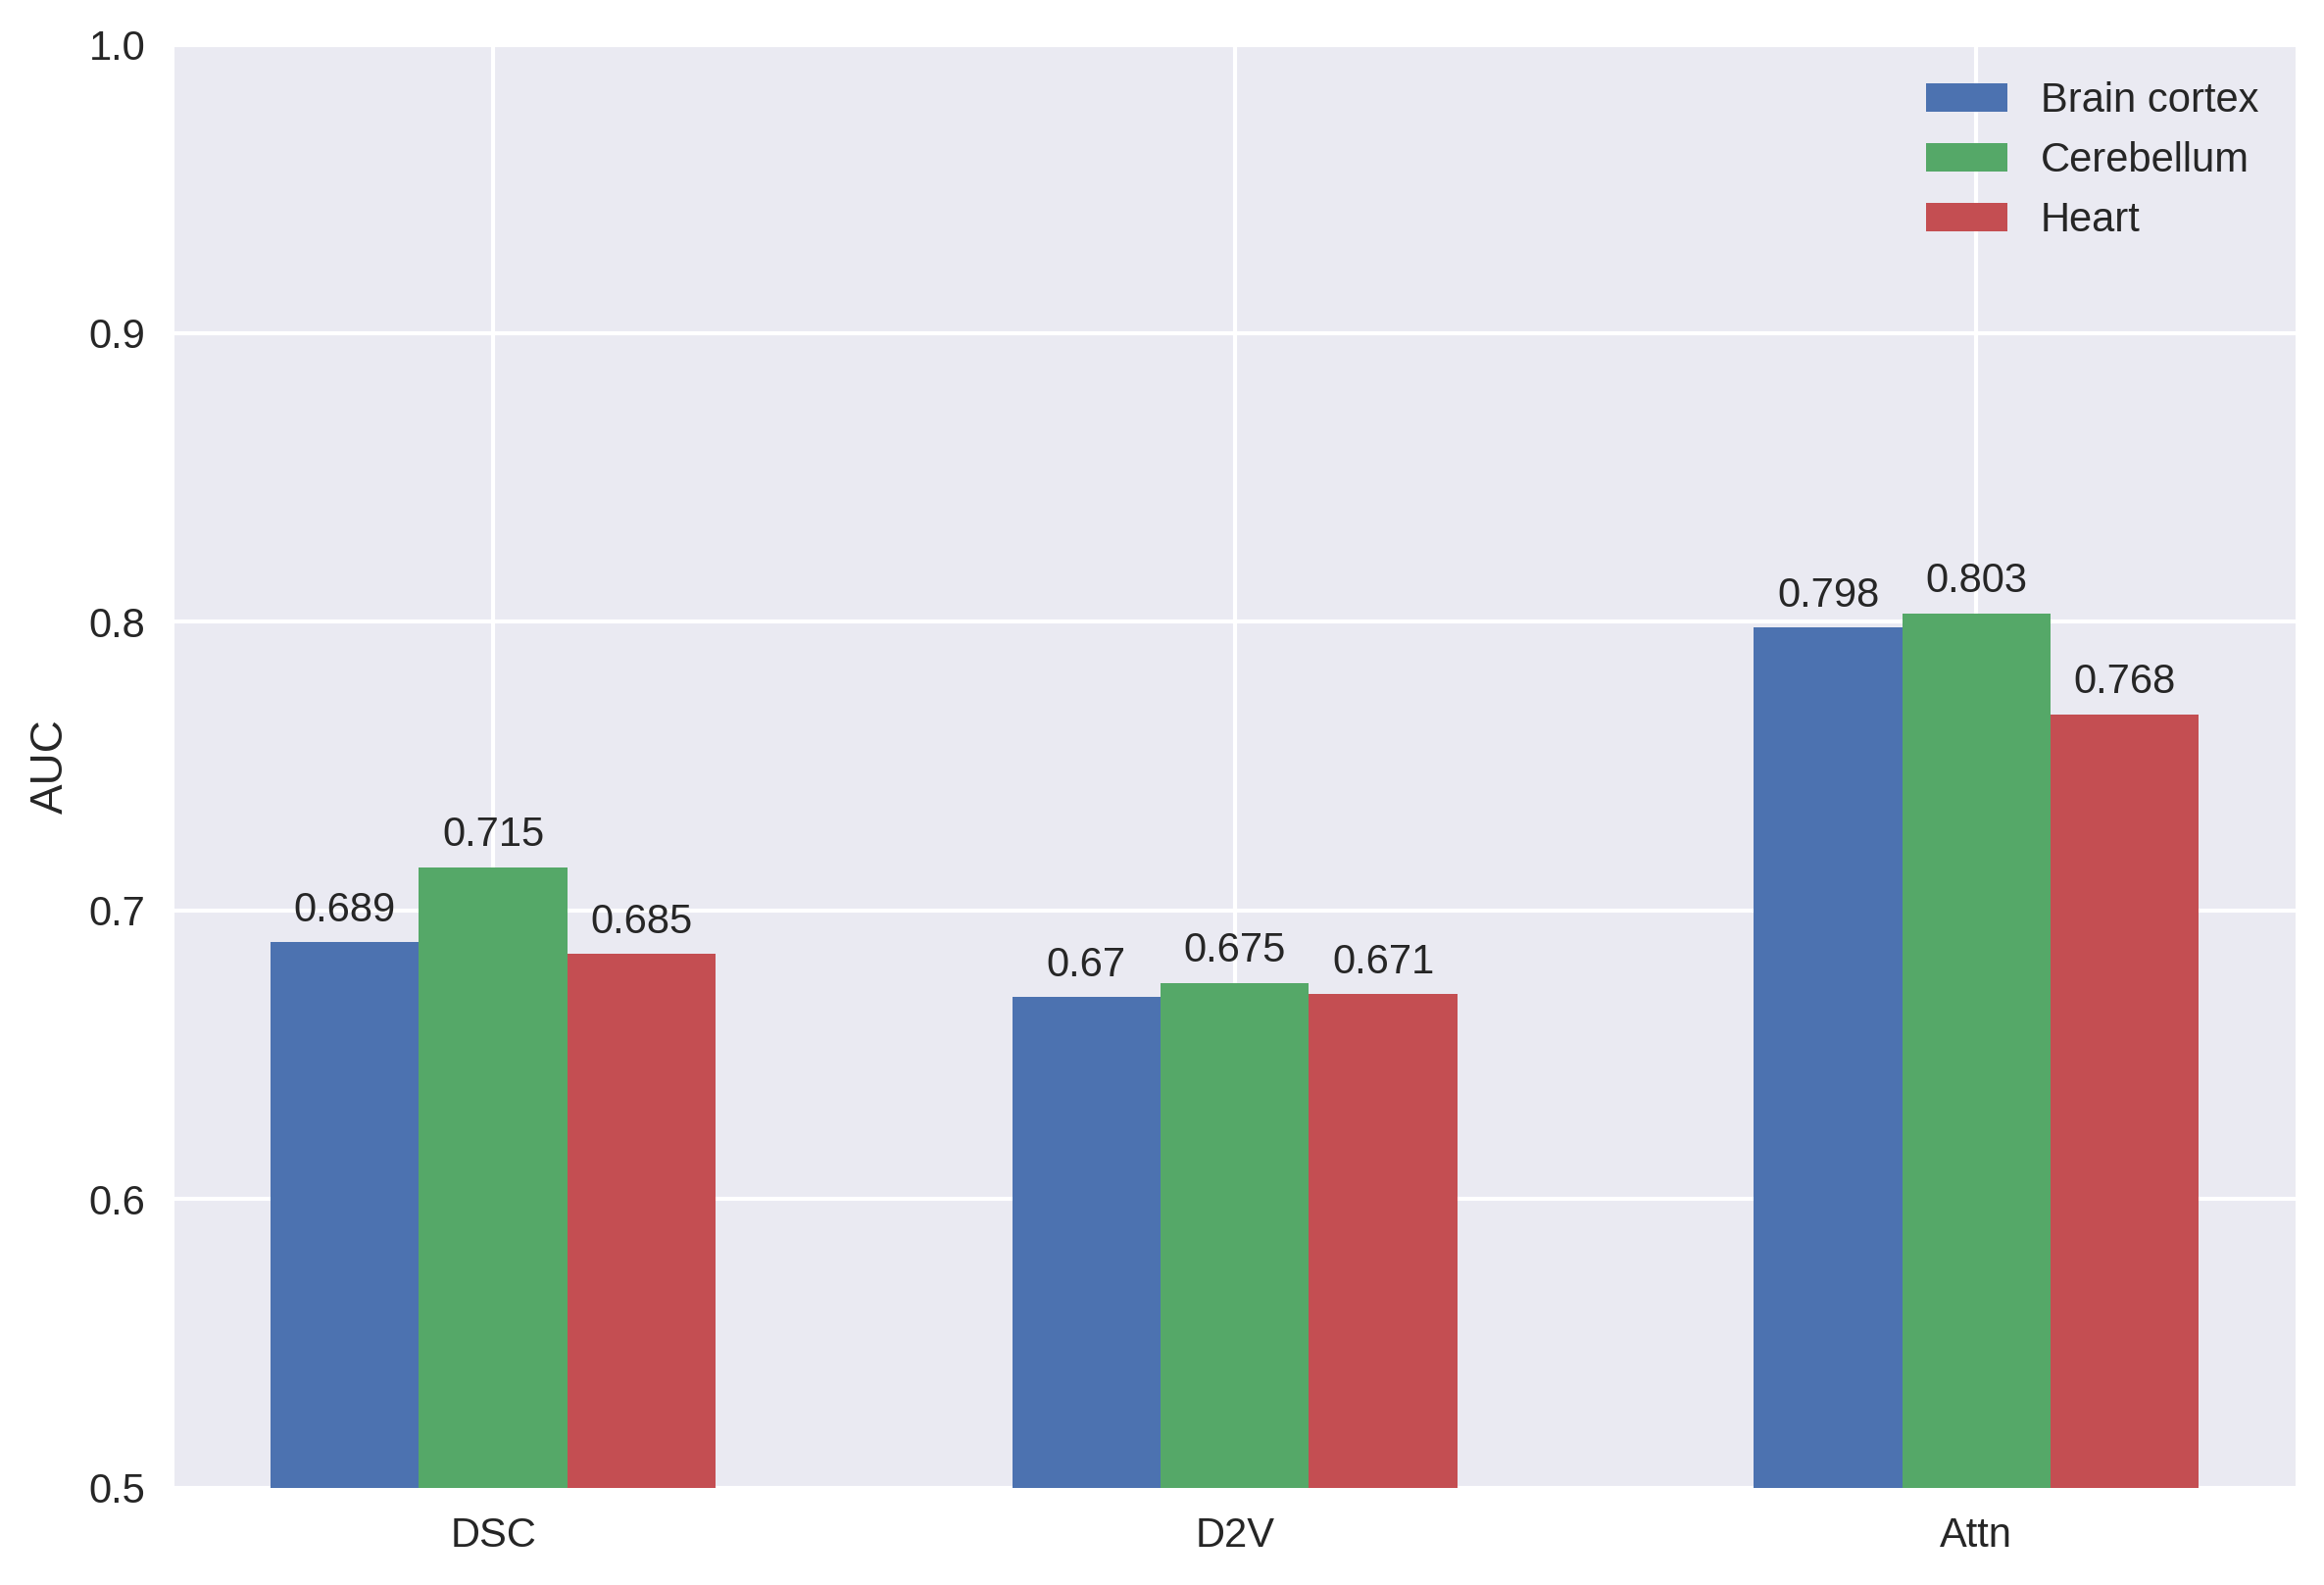
\includegraphics[width=0.7\textwidth]{../visualizations/gtex_junc_barcharts.png} 
	\caption{Performance on the GTEx-based junction datasets for different tissues. }
	\label{fig:gtex_junc_barcharts}
\end{figure}

\begin{figure}[h]
	\includegraphics[width=0.5\textwidth]{../saved/log/GTEx_Junc_Heart_DSC/final/ROC.png} 
	\includegraphics[width=0.5\textwidth]{../saved/log/GTEx_Junc_Heart_Attn/final/ROC.png}
	\caption{Left: ROC curve of the DSC model on heart tissue. Right: ROC curve of the Attn model on heart tissue. }
	\label{fig:gtex_junc_rocs}
\end{figure}

TODO: rerun these with cross-validation (will take ~30 hours of trainig time though)

- performance across the board a lot better; seemingly an easier task\\
- fairly clear correlation with more training samples -> more performance (cerebellum has most, heart has fewest)\\
- high / low difficulty trend doesn't really hold. 


\subsection{Reconstructing HEXEvent-dataset with GTEx data}
- dataset where I only took exons which were also in GTEx data
- seriously considering not showing these results as I basically already debunked HEXEvent at this point -- so from a narrative perspective, why spend effort on replicating it?



In \ref{subsubsec:naivepsi}, we mentioned issues when trying to estimate PSI naively. Although we tried to alleviate these as far as possible in pre-processing, we don't account for the information contained in non-junction reads and that from multiple samples. As a result, data quality is likely still an issue. Alleviating these issues, we next evaluate our models based on a primary data source which gives access to raw RNA-seq reads. This enables us to use methods from the literature which leverage information from non-junction reads and multiple samples.

\section{HipSci-based datasets} \label{sec:hipsci} 
\subsection{SUPPA with neuron tissue induced iPSCs} \label{subsec:hipsci_suppa}

\begin{figure}
	\centering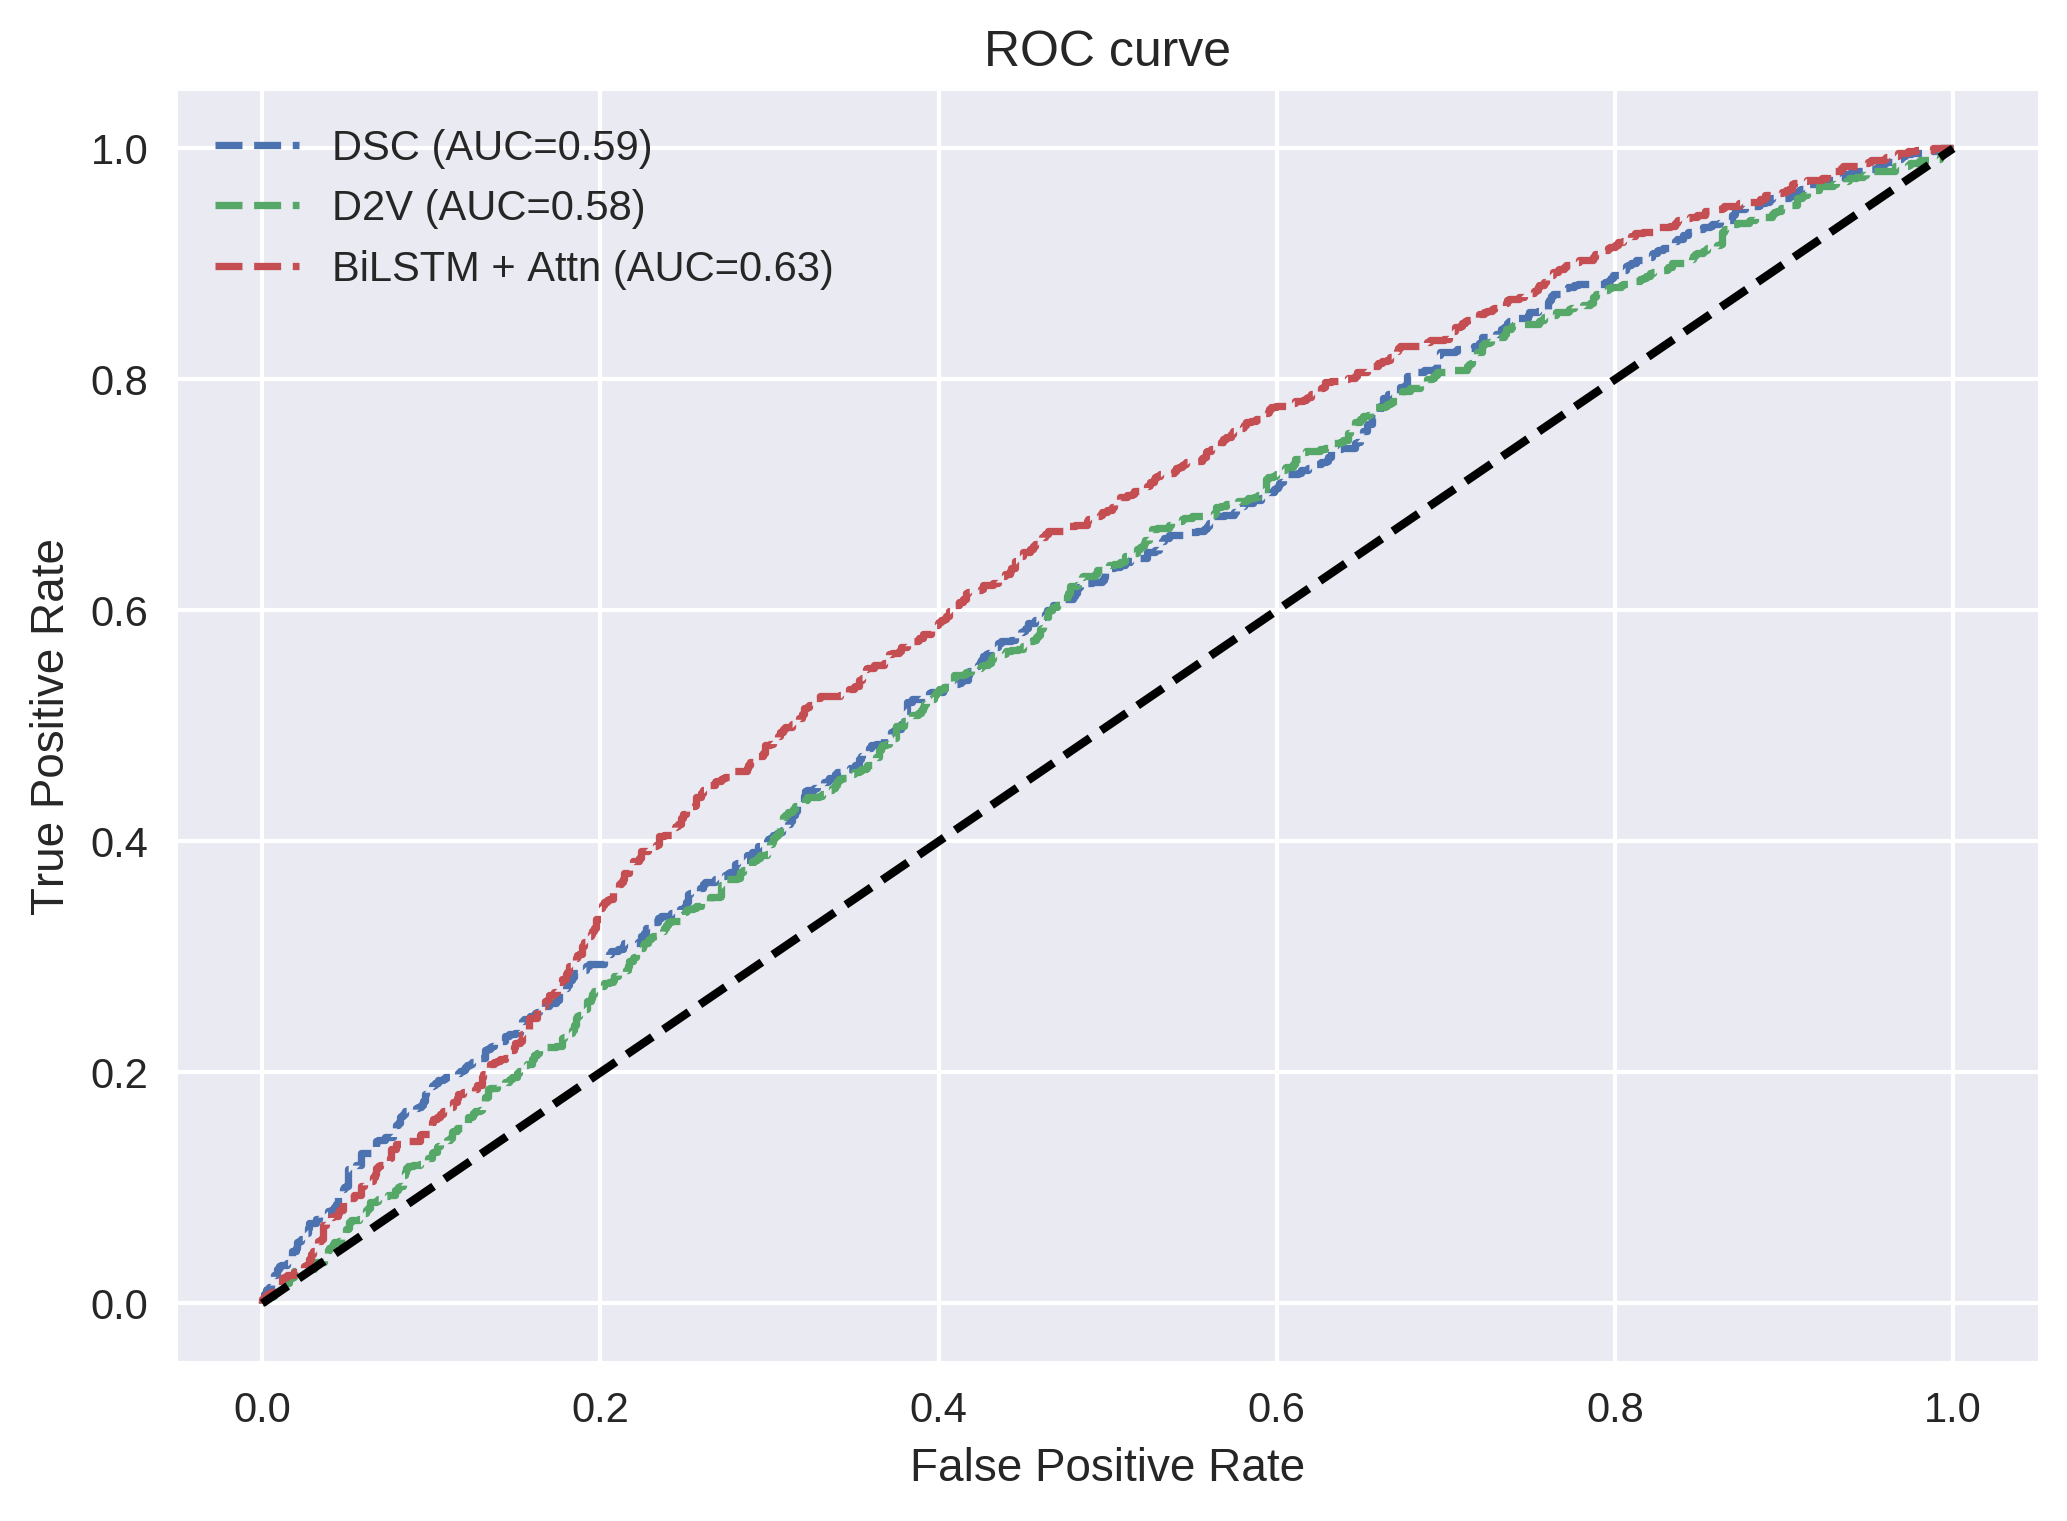
\includegraphics[width=0.7\textwidth]{../visualizations/suppa_cross_model_roc_auc_comparison.png} 
	\caption[bla.]{Comparison of the ROC curves of the three main models on the HipSci dataset derived by using SUPPA. }
	\label{fig:suppa_auc}
\end{figure}

Takeaways:
\begin{enumerate}
	\item All models perform similarly, BiLSTM + Attn tends to perform best
	\item All models perform very poorly perhaps a dataset issue (due to HIPSCI SUPPA being coarse-grained)
\end{enumerate}

\subsection{MAJIQ with iPSCs differentiated to neurons (exons)} \label{sec:hipsci_neuron_majiq}


\subsection{MAJIQ with iPSCs differentiated to neurons (junctions)}
haven't run experiments yet, not sure if results are interesting (but probably yes)\\
due to training times, probably don't want to run these with cross-validation as that would take 15 hours+


\subsection{MAJIQ with undifferentiated iPSCs} \label{subsec:hipsci_ipsc_majiq}



cross-tissue comparison here with very low variance across tissues;\\
seems like learned features are tissue-invariant\\


interpretation of attention mechanism etc follows here; some pretty graphics to follow